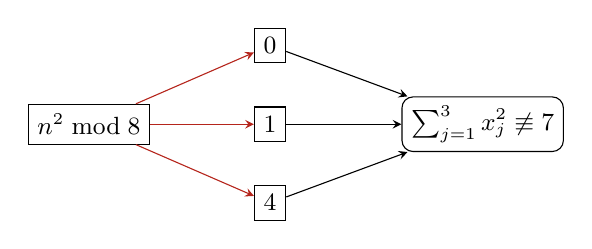
\begin{tikzpicture}[>=stealth,font=\small]
\node[draw] (a) at (0,0) {$n^2\bmod8$};
\node[draw] (b) at (2.3,1) {$0$};
\node[draw] (c) at (2.3,0) {$1$};
\node[draw] (d) at (2.3,-1) {$4$};
\node[draw,rounded corners] (e) at (5,0) {$\sum_{j=1}^3x_j^2\not\equiv7$};
\draw[->,BrickRed] (a)--(b);\draw[->,BrickRed] (a)--(c);\draw[->,BrickRed] (a)--(d);
\draw[->] (b)--(e); \draw[->] (c)--(e); \draw[->] (d)--(e);
\end{tikzpicture}
